\chapter{Analyse et spécification des besoins}

\section*{Introduction}
\addcontentsline{toc}{section}{Introduction }
    \par Le deuxième chapitre se consacre à l'analyse et à la spécification des besoins. Nous examinons en profondeur les besoins fonctionnels et non fonctionnels, tout en définissant clairement le flux de travail et le backlog du produit. Ces éléments constituent la base essentielle de la phase suivante de planification et de développement.

\section{Identification des besoins}
\par Dans cette section on va focaliser sur les besoins fonctionnels et non fonctionnels de notre projet.
    % Une sous section
    \subsection{Besoins fonctionnels}

        \par Cette section décrit en détail les besoins fonctionnels du projet de monitoring des opérations Snowflake.
        Ces besoins ont été identifiés à partir des exigences de l'entreprise et des utilisateurs, et sont essentiels pour le développement d'une solution efficace et adaptée aux besoins de l'entreprise.
    \begin{itemize}
            \item \textbf{Collecte automatique des données de performance de Snowflake} :
            Le système doit être capable de collecter automatiquement les données de performance de Snowflake, y compris les temps de réponse des requêtes, l'utilisation des ressources (CPU, mémoire, stockage) et les statistiques sur les entrepôts de données.
            
            \item \textbf{Surveillance en temps réel des requêtes SQL} :
            Le système doit surveiller en temps réel les requêtes SQL exécutées sur Snowflake, enregistrant les temps de réponse, les erreurs éventuelles, et en identifiant les requêtes lentes ou mal optimisées.
            
            \item \textbf{Surveillance en temps réel des entrepôts de données} :
            Le système doit surveiller en temps réel les métriques des entrepôts de données, y compris l'utilisation de l'espace disque, la répartition de la charge de travail et la consommation de ressources.
            
            \item \textbf{Tableaux de bord interactifs pour les métriques clés} :
            Le système doit fournir des tableaux de bord interactifs permettant de visualiser les métriques clés de performance de Snowflake, y compris les temps de réponse des requêtes, l'utilisation des ressources et les statistiques sur les entrepôts de données.
            
            \item \textbf{Suivi des tâches et des workflows (DAG monitoring)} :
            Le système doit permettre le suivi des tâches et des workflows exécutés sur Snowflake, enregistrant les étapes effectuées, les temps d'exécution et les erreurs éventuelles.
            
            \item \textbf{Surveillance de l'utilisation des crédits} :
            Le système doit surveiller l'utilisation des crédits de calcul sur Snowflake, enregistrant les crédits utilisés par chaque requête ou chaque tâche, ainsi que les tendances d'utilisation au fil du temps.
            
            \item \textbf{Surveillance des utilisateurs et des accès} :
            Le système doit suivre l'activité des utilisateurs sur Snowflake, en enregistrant les requêtes exécutées, les tables accédées et les autorisations utilisées.
            
            \item \textbf{Alertes et notifications en cas d'anomalies} :
            Le système doit générer des alertes et des notifications en temps réel en cas d'anomalies ou de situations critiques, telles qu'une augmentation soudaine du temps de réponse des requêtes ou une utilisation anormale des ressources.
            
            \item \textbf{Personnalisation des tableaux de bord} :
            Le système doit permettre aux utilisateurs de personnaliser les tableaux de bord en fonction de leurs besoins spécifiques, en sélectionnant les métriques à afficher et en configurant les seuils d'alerte.
        \end{itemize}        
    % Une deuxième sous section
    \subsection{Besoins non fonctionnels}
  \par Cette section détaille les besoins non fonctionnels du projet de monitoring des opérations Snowflake. 
  Ces besoins concernent principalement les aspects de performance, de sécurité, d'évolutivité et d'expérience utilisateur de la solution. Ils sont essentiels pour garantir que le système répond aux attentes de l'entreprise en termes de qualité et de fiabilité.

  \begin{itemize}
        \item\textbf{Besoins en Performance}

                \begin{enumerate}
                    \item[1.] \textbf{Temps de réponse} : Le système doit fournir des temps de réponse rapides pour l'affichage des tableaux de bord et la génération des rapports, afin de garantir une expérience utilisateur fluide.
                    
                    \item[2.] \textbf{Évolutivité} : Le système doit être capable de gérer une grande quantité de données et de trafic sans compromettre ses performances, en s'adaptant de manière transparente à l'augmentation de la charge.
                \end{enumerate}
    
        \item\textbf{Besoins en Sécurité}
    
                \begin{enumerate}
                    \item[1.] \textbf{Confidentialité des données} : Le système doit garantir la confidentialité des données collectées, en assurant leur cryptage lors du stockage et de la transmission.
                    
                    \item[2.] \textbf{Authentification et autorisation} : Le système doit mettre en place des mécanismes d'authentification robustes pour vérifier l'identité des utilisateurs et des administrateurs, ainsi que des contrôles d'autorisation pour limiter l'accès aux données sensibles.
                \end{enumerate}
    
        \item\textbf{Besoins en Disponibilité}
    
                \begin{enumerate}
                    \item[1.] \textbf{Disponibilité} : Le système doit être disponible en permanence, avec un temps de fonctionnement maximal et une reprise rapide en cas de panne.
                    
                    \item[2.] \textbf{Tolérance aux pannes} : Le système doit être capable de résister aux pannes matérielles ou logicielles, en assurant la redondance des composants critiques et la sauvegarde des données.
                \end{enumerate}
    
        \item\textbf{Besoins en Expérience Utilisateur}
    
                \begin{enumerate}
                    \item[1.] \textbf{Facilité d'utilisation} : Le système doit être intuitif et convivial, avec une interface utilisateur bien conçue et une navigation facile.
                    
                    \item[2.] \textbf{Personnalisation} : Le système doit permettre aux utilisateurs de personnaliser leur expérience, en configurant les préférences d'affichage et les paramètres de notification.
                \end{enumerate}
        \item \textbf{Archivage des données: }Les données historiques doivent être archivées de manière efficace pour garantir l'intégrité des données.
  \end{itemize}
  \section{Flux de travail}
  
  \par Durant la réalisation de notre projet, Ce processus a été notre fil conducteur, nous permettant de passer par plusieurs étapes clés pour atteindre notre objectif.
  La figure \textbf{\ref{fig:BPMN}} suivante illustre notre processus métier:
    %code image
        \begin{figure}[H]
        \centering
        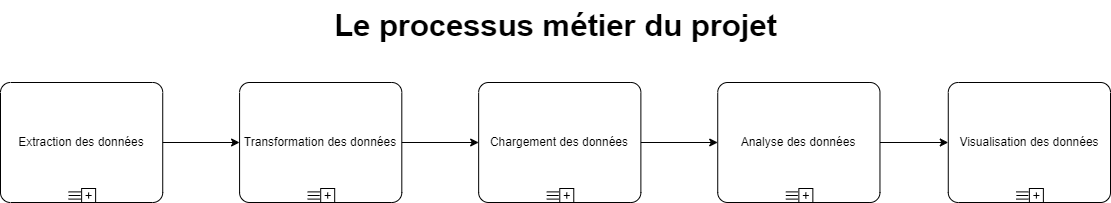
\includegraphics[width =1\linewidth , height=3.5cm]{img/conception/BPMN.png}
        \caption{Processus métier du projet}
        \label{fig:BPMN}
        \end{figure}
    %fin
  \par Dans cette partie, nous allons explorer en détail le flux de travail que nous avons suivi, en soulignant l'importance de chaque étape et en expliquant comment elles se sont complétées pour aboutir à une solution complète. Ensuite, nous examinerons chaque étape de manière approfondie pour comprendre comment elles ont contribué à notre succès global.
  \par Passons maintenant à l'examen détaillé de chacune de ces étapes.
  \begin{itemize}
  \item \textbf{Extraction des données: }
  \par Cette étape consistait à recueillir des informations provenant des différents vues du systéme de Snowflake.
\par L'objectif principal de cette étape était de collecter les données nécessaires à notre analyse. Les données brutes sont la matière première de toute analyse, et leur extraction était le point de départ de notre projet.
  \item \textbf{Transformation des données:}
  \par L'objectif principal de cette étape était de nettoyer et de structurer les données. Les données brutes extraites pouvaient contenir des erreurs, des doublons, des incohérences et des valeurs manquantes. La transformation des données avait pour but de les rendre utilisables, fiables et cohérentes.
   \item \textbf{Chargement des données:}
  \par Une fois les données nettoyées et préparées, elles sont acheminées vers une base de données ou un entrepôt de données, comme PostgreSQL dans notre projet. Le chargement vise à stocker les données de manière centralisée pour une accessibilité et une analyse ultérieures.
   \item \textbf{Analyse des données :}
  \par Cette phase consiste à explorer les données pour en extraire des informations significatives. On utilise des méthodes statistiques, des techniques de modélisation, des calculs de corrélation, etc., pour comprendre les tendances et les relations entres les données.
   \item \textbf{Visualisation des données}:
  \par L'analyse des données est souvent présentée de manière visuelle sous forme de tableaux de bord interactifs, de graphiques, de diagrammes et d'autres représentations graphiques. Ces visualisations permettent aux utilisateurs de comprendre rapidement les résultats de l'analyse.
  \end{itemize}
  \par Ces phases constituent un flux de travail complet pour gérer les données, les transformer en informations exploitables et les présenter de manière efficace pour aider nos utilisateurs finaux à surveiller leurs données d'une maniére concrête.
\section{Le backlog du produit}
\par Le backlog de produit est destiné à recueillir tous les besoins du client pour l'équipe projet. Il contient la liste des fonctionnalités inclues dans un produit, ainsi que les éléments nécessitant l’intervention de l’équipe projet. Le backlog Scrum classe les éléments par priorité pour indiquer leur ordre de réalisation.\cite{blog}.

 \par Le backlog en KANBAN n’est pas si différent d’un backlog scrum en réalité. La différence réside surtout sur les règles de sa gestion. Bien que le scrum reste évasif sur le sujet, il rappelle quelques règles importantes. \cite{BPK}  
    
    \par la table \textbf{\ref{tab:backlog_produit}} suivante présente le backlog de produit de notre projet. 
%%%%%table
\begin{center}

    \begin{longtable}{|p{0.05\linewidth}|p{0.65\linewidth}|p{0.12\linewidth}|p{0.12\linewidth}|}
        \hline       
        \rowcolor{blue!18}\textbf{ID} & \textbf{User Story} &  \textbf{Priorité} & \textbf{Estimation (points)} \\
        \hline
        \endfirsthead
        US1 &  En tant qu'utilisateur, je veux un tableau de bord global pour surveiller les performances générales de l'entrepôt de données, y compris les temps de réponse des requêtes, l'utilisation des ressources et les erreurs éventuelles. & Haute & 8 \\
        
        \hline
        
        US2 &  En tant qu'administrateur, je veux être en mesure de suivre en temps réel l'exécution des requêtes SQL sur la plateforme Snowflake, y compris les temps d'exécution, le nombre de lignes retournées et les plans d'exécution. & Haute & 10 \\
        
        \hline
        
        US3 &  En tant qu'administrateur, je veux surveiller l'utilisation des ressources (CPU, stockage, etc.) de l'entrepôt de données pour identifier les goulots d'étranglement et les problèmes de capacité. & Haute & 9 \\
        
        \hline
        
        US4 &  En tant qu'administrateur, je veux recevoir des alertes en temps réel en cas de dégradation des performances de l'entrepôt de données afin de pouvoir réagir rapidement et résoudre les problèmes. & Haute & 8 \\
        
        \hline
        
        US5 & En tant qu'utilisateur, je veux générer des rapports de charge pour analyser la consommation de crédits, le coût par requête et l'utilisation des ressources au fil du temps. & Moyenne & 6 \\
        
        \hline
        
        US6 &  En tant qu'administrateur, je veux suivre l'activité des utilisateurs sur la plateforme Snowflake, y compris les requêtes exécutées, les tables accédées et les autorisations utilisées. & Moyenne & 7 \\
        
        \hline
        
        US7 &  En tant qu'administrateur, je veux être capable de gérer les sessions utilisateur actives, y compris la déconnexion des sessions inactives et la surveillance des sessions gourmandes en ressources. & Haute & 8 \\
        
        \hline
        
        US8 &  En tant qu'administrateur, je veux pouvoir définir des alertes personnalisées basées sur des seuils de performance spécifiques pour les requêtes, les ressources et les sessions. & Moyenne & 7 \\
        
        \hline
        
        US9 &  En tant que développeur, je veux accéder à des recommandations d'optimisation des requêtes SQL pour améliorer les performances et réduire les coûts. & Faible & 9 \\
        
        \hline
        
        US10& En tant qu'administrateur, je veux surveiller l'exécution des tâches planifiées (comme les pipelines de chargement) pour détecter les retards ou les échecs. & Moyenne & 6 \\
        
        \hline
        
        US11 & En tant qu'utilisateur, je veux pouvoir analyser les tendances historiques des performances pour identifier les schémas et les anomalies. & Moyenne & 8 \\
        
        \hline
        
        US12 & En tant qu'utilisateur, je veux s'authentifier d'une façon sécurisée pour accéeder a la platforme de monitoring & Moyenne & 5 \\
        
        \hline
        US13 & En tant qu'administrateur, je veux suivre en temps réelle l'execution des taches programmés  & haute & 13 \\
        
        \hline
        
        \caption{Backlog de Produit}
        \label{tab:backlog_produit}
    \end{longtable}

\end{center}


%%%%%table
\vspace{-1cm}
\section*{Conclusion}
\addcontentsline{toc}{section}{Conclusion}
 Au terme de ce chapitre, nous avons obtenu une vision approfondie des besoins inhérents au projet. Cette analyse détaillée assure que notre solution est en phase avec les attentes et les exigences d'Avaxia Group. Dans le prochain chapitre, nous explorerons les aspects architecturaux et conceptuels de notre projet.